% !TeX document-id = {aa35f1f4-a045-449b-a615-5ff5efe1e0df}
% !TeX root = report_g1_p1.tex
% !TeX program = pdflatex
% !BIB program = biber
 %%%%%%%%%%%%%%%%%%%%%%%%%%%%%%%%%%%%%%%%%%%%%%%%%%%%%%%%%%%%%%%%%%%%%%%%%%%%%%%%
 % Template for USENIX papers.
 %
 % History:
 %
 % - TEMPLATE for Usenix papers, specifically to meet requirements of
 %   USENIX '05. originally a template for producing IEEE-format
 %   articles using LaTeX. written by Matthew Ward, CS Department,
 %   Worcester Polytechnic Institute. adapted by David Beazley for his
 %   excellent SWIG paper in Proceedings, Tcl 96. turned into a
 %   smartass generic template by De Clarke, with thanks to both the
 %   above pioneers. Use at your own risk. Complaints to /dev/null.
 %   Make it two column with no page numbering, default is 10 point.
 %
 % - Munged by Fred Douglis <douglis@research.att.com> 10/97 to
 %   separate the .sty file from the LaTeX source template, so that
 %   people can more easily include the .sty file into an existing
 %   document. Also changed to more closely follow the style guidelines
 %   as represented by the Word sample file.
 %
 % - Note that since 2010, USENIX does not require endnotes. If you
 %   want foot of page notes, don't include the endnotes package in the
 %   usepackage command, below.
 % - This version uses the latex2e styles, not the very ancient 2.09
 %   stuff.
 %
 % - Updated July 2018: Text block size changed from 6.5" to 7"
 %
 % - Updated Dec 2018 for ATC'19:
 %
 %   * Revised text to pass HotCRP's auto-formatting check, with
 %     hotcrp.settings.submission_form.body_font_size=10pt, and
 %     hotcrp.settings.submission_form.line_height=12pt
 %
 %   * Switched from \endnote-s to \footnote-s to match Usenix's policy.
 %
 %   * \section* => \begin{abstract} ... \end{abstract}
 %
 %   * Make template self-contained in terms of bibtex entires, to allow
 %     this file to be compiled. (And changing refs style to 'plain'.)
 %
 %   * Make template self-contained in terms of figures, to
 %     allow this file to be compiled. 
 %
 %   * Added packages for hyperref, embedding fonts, and improving
 %     appearance.
 %   
 %   * Removed outdated text.
 %
 %%%%%%%%%%%%%%%%%%%%%%%%%%%%%%%%%%%%%%%%%%%%%%%%%%%%%%%%%%%%%%%%%%%%%%%%%%%%%%%%
 
 \documentclass[letterpaper,twocolumn,10pt]{article}
 \usepackage{usenix}
 \usepackage[backend=biber, sorting=none]{biblatex}
 \addbibresource{report_g1_p1.bib}

 
 % to be able to draw some self-contained figs
 \usepackage{tikz}
 \usetikzlibrary{
  arrows.meta,
  positioning,
  fit,
  calc
}
 \usepackage{amsmath}
 \usepackage{listings}

 \usepackage[acronym]{glossaries}
 \makeglossaries 
 \newacronym{pgo}{PGO}{Profile Guided Optimization}
 \newacronym{ir}{IR}{Intermediate Representation}
 \newacronym{simd}{SIMD}{Single Instruction Multiple Data}
 \newacronym{mca}{MCA}{Machine Code Analyzer}
 \newacronym{smt}{SMT}{Satifiablility Module Theories}
 \newacronym{ssa}{SSA}{Static Single-Assignment}

 %-------------------------------------------------------------------------------
 \begin{document}
 	%-------------------------------------------------------------------------------

 	%don't want date printed
 	\date{}
 	
 	% make title bold and 14 pt font (Latex default is non-bold, 16 pt)
 	\title{\Large \bf Correct Optimizations: Phase 2 Report Based on \citetitle{liu24:minotaur} \cite{liu24:minotaur}}
 	
 	%for single author (just remove % characters)
 	\author{
 		{\rm Kilian Schulz}\\
 		Technical University Munich
 		\and
 		{\rm Ilja Gamza}\\
 		Technical University Munich
 		\and
 		{\rm Tomás Gaspar}\\
 		Technical University Munich
 	} % end author
 	
 	\maketitle
 	
 	% %-------------------------------------------------------------------------------
 	% \begin{abstract}
 	% %-------------------------------------------------------------------------------
 	% 	TODO
 	% \end{abstract}
 	
 	
 	\section{Introduction}
	% What is the problem?
	% Why is it important or interesting?
	Minotaur \cite{liu24:minotaur} is a superoptimizer, that after computing optimizations, caches those in a data base.
	These optimizations consist of a key, which is the original code, and a value, which is an equivalent, but faster, rewrite of the original code.
	This caching is done in order to reduce the substantial runtimes of Minotaur for future compilations of the same or a similar program.
	Minotaurs compile times, with a cold cache, can easily be hundreds of time slower than with regular LLVM \cite{liu24:minotaur}.
	
	% What is the state-of-the-art? What is the research-gap?
	% Current state in Minotuar
	Currently Minotaur directly uses the extracted code segments in LLVM IR as the keys and stores those along side a rewrite, in Minotaurs own IR as value, in the cache as shown in example \ref{fig:kv}.

			\begin{figure*}[t]
		\centering
		\caption{\label{fig:kv} Example of a key value pair as it is found in the Minotaur cache.}
		\begin{lstlisting}[language=llvm, basicstyle=\small\tt]
		key:
			define i1 @cut(i64 %__n2, i16 %__n3) {
				%__n0 = sub nsw i64 0, %__n2
				%__n1 = icmp samesign ult i64 %__n0, 2033
				ret i1 %__n1
			}
		\end{lstlisting}
		\begin{lstlisting}[basicstyle=\small\tt]
		value:
			(icmp_sgt (var i64 %__n2) (reservedconst i64 |i64 -2033|) b1)	
		\end{lstlisting}
	 	\end{figure*}


	This approach can easily lead to near misses, where an equivalent code segment is already cached, but for instance has unused arguments, leading to a cache miss and a costly recompute of an optimization.
	% To mitigate this we extended Minotaur \cite{liu24:minotaur} to support key canonicalization through multiple steps.

	% Why is it difficult? What are the challenges?
	One way to avoid this issue is to attempt to increase the number of cache hits while keeping the correctness of the mapping between keys and their rewrite.
	This leads to reduced compile times of Minotaur even when starting from a cold cache.

	\section{Research Proposal}
	% What is the proposed solution?
	% How it works at a high-level?
	Our solution introduces an additional step after the cut extraction.
	It performs multiple code transformations, with the goal of reducing the number of possible equivalent keys, mapping those to one canonicalized key.

	% What are the key insights?
	% What are novel aspects?
	The idea is that this leads to fewer cache entries, increasing the cache hit rate and reducing the number of slow optimization searches by Minotaur.
	For large enough projects this can already take effect during a build even when starting with an empty cache thereby reducing compile time.

	\section{Canonicalization}
	Our extended version of Minotaur is available on GitHub \footnote{\href{https://github.com/KiSchulz/minotaur}{Extended Minotaur Version}}.

	% How did you design and implement the system?
	% TODO: look into https://github.com/llvm/llvm-project/tree/main/llvm/tools/llvm-reduce
	The canonicalizer is placed as a pre- and postprocessing step around Minotaurs inference step.
	We intercept the LLVM IR produced by the slicer and perform transformations on it to produce a canonicalized version of the input which is then forwarded to the inference step.
	In the following this transformation is called canonicalization.
	After the inference step is finishes and returns a rewrite (in Minotaurs own IR), the canonicalizer again performs transformations on the rewrites.
	This process is called de-canonicalization.
	The structure of the augmented Minotaur with our canonicalizer is shown in figure \ref{fig:architecture}.	

	% TODO add a figure ilustrating our canonicalization steps to support this paragraph
	Each canonicalization-step in our implementation consists of a canonicalization function and a de-canonicalization function.
	The canonicalization-steps are ordered as to not interfere with each other.
	More on that is discussed in section \ref{sec:ordering}.
	During the canonicalization process every canonicalization function is applied iteratively in this predefined order.
	% TODO: talk about why we need the reverse order
	For de-canonicalization the de-canonicalization functions are applied in the reverse order in which the canonicalization-steps are specified.
	It is also possible to pass information between the pairs of canonicalization and de-canonicalization functions of each step if required.
	This enables the support for more complex transformations.

	\begin{figure*}[t]
		\begin{center}
			\caption{\label{fig:architecture} Structure of Minotaur and how the Canonicalization is integrated. The highlighted blocks were added for (De-)Canonicalization.}
			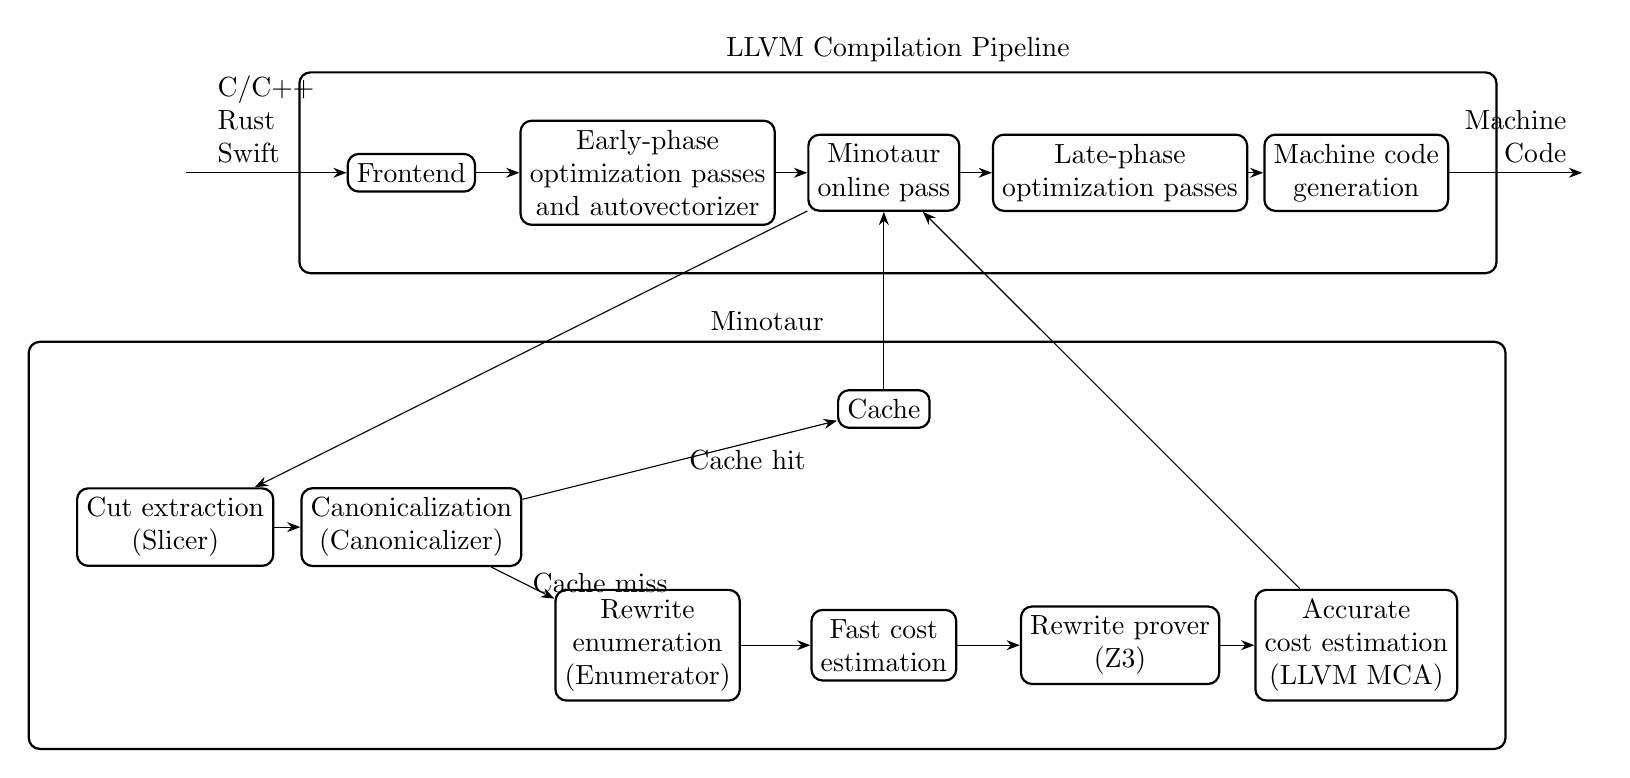
\begin{tikzpicture}
% -------------------------
% Nodes
% -------------------------
\begin{scope}[
  every node/.style={draw, rounded corners, thick, align=center}
]

% Invisible start / end
\node[draw=none] (start) at (-3, 0) {};
\node[draw=none] (end)   at (15, 0) {};

% LLVM pipeline
\node (frontend) at (0, 0)   {Frontend};
\node (opt1)     at (3, 0)   {Early-phase\\optimization passes\\and autovectorizer};
\node (minotaur) at (6, 0)   {Minotaur\\online pass};
\node (opt2)     at (9, 0)   {Late-phase\\optimization passes};
\node (backend)  at (12, 0)  {Machine code\\generation};

% Minotaur internals
\node (slicer)     at (-3, -4.5) {Cut extraction\\(Slicer)};
\node (canon)      at (0, -4.5) {Canonicalization\\(Canonicalizer)};
\node (cache)      at (6, -3) {Cache};

\node (enumerator) at (3, -6)   {Rewrite\\enumeration\\(Enumerator)};
\node (fastcost)   at (6, -6)  {Fast cost\\estimation};
\node (prover)     at (9, -6)  {Rewrite prover\\(Z3)};
\node (llvmMCA)    at (12, -6)  {Accurate\\cost estimation\\(LLVM MCA)};

\end{scope}

% -------------------------
% Edges
% -------------------------
\begin{scope} [>={Stealth[black]}]
% External inputs / outputs
\path [->] (start) edge node[above, align=left] {C/C++\\Rust\\Swift} (frontend);
\path [->] (backend) edge node[above, align=right] {Machine\\Code} (end);

% LLVM pipeline
\path [->] (frontend) edge (opt1);
\path [->] (opt1)     edge (minotaur);
\path [->] (minotaur) edge (opt2);
\path [->] (opt2)     edge (backend);

% Minotaur pipeline
\path [->] (minotaur) edge (slicer);
\path [->] (slicer)   edge (canon);

\path [->] (canon) edge node[right]{Cache miss} (enumerator);
\path [->] (enumerator) edge (fastcost);
\path [->] (fastcost)   edge (prover);
\path [->] (prover)     edge (llvmMCA);
\path [->] (llvmMCA)    edge (minotaur);

\path [->] (canon) edge node[right]{Cache hit} (cache);
\path [->] (cache) edge (minotaur);

\end{scope}

% -------------------------
% Clusters (boxes)
% -------------------------
\node[
  draw,
  thick,
  rounded corners,
  fit=(frontend)(opt1)(minotaur)(opt2)(backend),
  label=above:{LLVM Compilation Pipeline},
  inner sep=6mm
] {};

\node[
  draw,
  thick,
  rounded corners,
  fit=(slicer)(canon)(cache)(enumerator)(fastcost)(prover)(llvmMCA),
  label=above:{Minotaur},
  inner sep=6mm
] {};

\end{tikzpicture}


		\end{center}
	\end{figure*}

	\subsection{Canonicalization Steps \label{sec:steps}}
	% TODO: talk about what equivalent means here
	% TODO: fix this version of equivalence since it does not quite work for changes in signature
	% TODO: talk about that each step reduces the size of the key space and also add this to each prove
	% TODO: explain what the depth of function is
	In the following we explain each canonicalization-step.
	We selected our steps such that each step is correct, productive and does not modify the functions depth.
	Correctness means that both the canonical function and the original function applied to the same arguments compute the same result( and have the same effect on memory also with respect to order of memory operation).
	A step is productive iff it reduces the size of the space of all possible keys after the step is applied.
	%The depth is kept constant as increasing this has a large impact on runtime as shown in original paper \cite{liu24:minotaur}.

	Those criteria were chosen to only allow for simple transformation steps.
	It might be possible to relax the correctness definition.
	Similarly the definition of productivity could be relaxed such that it only holds over all steps but not for every individual step.
	Also the depth constraint is not strictly required and could be dropped, but this would likely result in more complex  solver queries which could drastically impact the overall build times.
	This issue was already explored in the original paper \cite{liu24:minotaur}.
	
	An example of all the steps applied sequentially to an example input is shown in figure \ref{fig:canon_full}

	\begin{figure*}[t]
\centering
\caption{\label{fig:canon_full} Example applying canonicalization steps (changes highlighted).}
\begin{minipage}[t]{\columnwidth}
\begin{lstlisting}[language=llvm, escapechar=!, basicstyle=\footnotesize\tt, columns=flexible]
input/key:
define i1 @cut(i32 %a, float %b, i32 %c,
		float %d) {
	%1 = fcmp uge float %b, %d
	%2 = icmp sle i32 %c, 15
	%3 = and i1 %1, %2
	%4 = and i1 %3, 0
	ret i1 %4
}
1. unused argument elimination:	
define i1 @cut !\colorbox{blue!50}{(float \%b, i32 \%c, float \%d)}! {
	%1 = fcmp uge float %b, %d
	%2 = icmp sle i32 %c, 15
	%3 = and i1 %1, %2
	%4 = and i1 %3, 0
	ret i1 %4
}
2. replacing greater-than with less-than:	
define i1 @cut(float %b, i32 %c, float %d) {
	%1 = fcmp !\colorbox{blue!50}{ule}! float %d, %b
	%2 = icmp sle i32 %c, 15
	%3 = and i1 %1, %2
	%4 = and i1 %3, 0
	ret i1 %4
}
\end{lstlisting}
\end{minipage}
\begin{minipage}[t]{\columnwidth}
\begin{lstlisting}[language=llvm, escapechar=!, basicstyle=\footnotesize\tt, columns=flexible]
3. replacing non-strict operators:	
define i1 @cut(float %b, i32 %c, float %d) {
	%1 = fcmp ule float %d, %b
	%2 = icmp !\colorbox{blue!50}{slt}! i32 %c, 16
	%3 = and i1 %1, %2
	%4 = and i1 %3, 0
	ret i1 %4
}
4. sorting arguments:
define i1 @cut!\colorbox{blue!50}{(float \%d, float \%b, i32 \%c)}! {
	%1 = fcmp ule float %d, %b
	%2 = icmp slt i32 %c, 16
	%3 = and i1 %1, %2
	%4 = and i1 %3, 0
	ret i1 %4
}
5. renaming argument:	
define i1 @cut !\colorbox{blue!50}{(float \%\_\_canonArg, float \%\_\_canonArg1,}!
		 !\colorbox{blue!50}{i32 \%\_\_canonArg2)}! {
	%1 = fcmp ule float %__canonArg, %__canonArg1
	%2 = icmp slt i32 %__canonArg2, 16
	%3 = and i1 %1, %2
	%4 = and i1 %3, 0
	ret i1 %4
}
output/value:
(reservedconst i1 |i1 false|)
\end{lstlisting}
\end{minipage}
\end{figure*}


	\paragraph{Replacing Greater-Than with Less-Than}
	A single comparison operation often has multiple semantically equivalent ways of being expressed.
	To address this we replace every greater-than or greater-equal comparison with a less-than or less-equal comparison respectively.
	For correctness we also have to swap the order of operands.
	\begin{align*}
		\forall x \forall y . (x\ P\ y \iff y\ P'\ x) \\
		with (P, P') \in {(>, <), (\geq, \leq)}
	\end{align*}
	This reduces the size of the key space since now only less-than and less-equal comparisons are performed.
	It also does not change the depth of the function.

	\paragraph{Non-strict Operator Replacement}
	The idea is to reduce the number of comparison operators that are available in order to decrease the number of possible way to express a comparison operation.
	This is done by replacing non-strict comparison operators like $\leq$ with $<$.
	To introduce additional operations this is only done when a constant is one of the operands.
	This constant is then adjusted accordingly if no prevented by an edge case like the constant being already the maximum or minimum value possible for the data type.
	So given some expression like $ x \leq c$ it would be transformed into $ x < c + \epsilon$ where $\epsilon$ is the smallest possible increment possible for $c$.
	% TODO: under which structure does this hold
	% TODO: define structure/theory?
	% TODO: explain further for floating point types
	\[
		\exists v \exists \epsilon \forall x . (( v = c + \epsilon) \implies (x \leq c \iff  x < c + \epsilon))
	\]
	An analogous argument can be made for the $\geq$ and for a swapped operands and works for both integral and floating point types.
	Currently vector types are filtered.

	\paragraph{Elimination of Unused Function Arguments}
	Some function have unused arguments.
	% TODO explain how values are represented in the cache so the last part of this sentence makes sense
	Those can simply be eliminated during the forward pass.
	% \\\textbf{Forward Pass:}
	Assuming the given input function $f$ has an unused argument we can define the following.
	Let $f: T_1 \times ... \times T_i \times ... \times T_n \to R$ and $g: T_1 \times ... \times T_{i-1} \times T_{i+1} \times ... \times T_n \to R$ be $n$-ary and $n-1$-ary functions respectively with
	\[
		f(t_1, ..., t_n) := g(t_1, ..., t_{i-1}, t_{i+1}, ..., t_n), t_j \in T_j
	\]
	Since $t_i$ is not part of the function signature of $g$ we can define a new function $f' := g$.
	This obviously does not change what is computed since
	\begin{align*}
		f(t_1, ..., t_n) &= g(t_1, ..., t_{i-1}, t_{i+1}, ..., t_n) \\
						 &= f'(t_1, ..., t_{i-1}, t_{i+1}, ..., t_n)
	\end{align*}
	% TODO: talk about why we can modify the function signature and why this usually can not be done
	Due to the implicit nature of the function signature in the values of the cache and the structure of Minotaur no additional work is required in relation to this step.

	\paragraph{Sorting of Function Arguments}
	Another modification that is done to the function signature is that we sort the arguments.
	The arguments are sorted by type-name and internally by when they are used inside the function body.
	Sorting by the type name is done in order to avoid cases where the function body is the same but a cache miss occurs due to the order of the types being different.
	To achieve a total order on the function arguments, each set of arguments of the same type are sorted by when they are used in the function body.
	This makes the argument order dependent on the function body and has to be taken into account when ordering the canonicalization steps.
	% This step also does not require any backward pass.
	The correctness of the step is shown in the following.
	Let $f: T_1 \times ... \times T_n \to R$ be the input function and $f': T_{\rho{(1)}} \times ... \times T_{\rho{(n)}} \to R$ the output function with $\rho: [n] \to [n]$ being a bijective function i.e. a permutation.
	We define 
	\begin{align*}
		f'(t_{\rho{(1)}}, ..., t_{\rho{(n)}}) &:= f(t_{\rho^{-1}{(\rho{(1)})}}, ..., t_{\rho^{-1}{(\rho{(n)})}}) \\
										  &= f(t_1, ..., t_n), t_i \in T_i \\ 
	\end{align*}
	This clearly shows that $f$ and $f'$ compute the same for all inputs.
	Similar to the elimination of unused arguments no further work is required.

	\paragraph{Renaming of Function Arguments}

	\subsection{Ordering of the Canonicalization Steps \label{sec:ordering}}
	% Describe the order in which the steps are applied and explain why
	% first greater... to less... change then argument ordering then argument renaming

	It is important to order the canonicalization-steps such that they do not interfere with previous once.
	In our case this is still relatively simple since we only have two constraints.

	First, the argument renaming step should be run after the last modification to functions arguments.
	In our case this implies that it has to run after the elimination of unused arguments step and after the argument sorting step.

	Second, the sorting of function arguments has to take place after the last modification to the function body in which the usage order of the arguments is changed.
	This means concretely that it has to be run after the step replacing greater than with less than operators.

	Based on those two constraints we can define the following order:

	\begin{enumerate}
		\item Replacing Greater-Than with Less-Than
		\item Non-strict Operator Replacement
		\item Elimination of unused Function Arguments
		\item Sorting of Function Arguments
		\item Renaming of Function Arguments
	\end{enumerate}
	
	\subsection{Issues with the original version}
	% Some of the debugging we did in the mean time.

	% TODO describe the order of the steps
	% TODO consider not adding this due to space constraints

	\section{Evaluation}
	\subsection{Setup}
	% hardware and general setup of the tests
	For the evaluation we used an AMD Ryzen 9 5900 CPU which has 12 cores running at up to 4.8 GHz .

	% what was done for each benchmark run
	Each benchmarked program was build once using Minotaur with canonicalization disabled and once with canonicalization enabled.
	Since our canonicalization steps are compositional we measured the effect each step and combination of steps have.
	Furthermore, we ran the provided tests and benchmarked each compiled program.

	% what was benchmarked and why
	We chose to benchmark libgmp-6.2.1 as the original paper did.
	Due to the long compile times experienced on libYUV, we decided against benchmarking it, like the original paper did, and instead opted to select different smaller projects.
	% TODO: mention the other projects that were benchmarked

	\subsection{Results}
	% Evaluation results
	% just the results no interpretation

	\section{Discussion}
	% Key findings
	% interpretation/explanation of the results

	\section{Future Work}
	% perform load ordering so between loads and also where to load data in a function e.g. at the beginning or end

	\section{Conclusion}
	% did it work, what issues are remaining, future work
 	
	\printbibliography
 	
 	%%%%%%%%%%%%%%%%%%%%%%%%%%%%%%%%%%%%%%%%%%%%%%%%%%%%%%%%%%%%%%%%%%%%%%%%%%%%%%%%
 \end{document}
 %%%%%%%%%%%%%%%%%%%%%%%%%%%%%%%%%%%%%%%%%%%%%%%%%%%%%%%%%%%%%%%%%%%%%%%%%%%%%%%%
 
 %%  LocalWords:  endnotes includegraphics fread ptr nobj noindent
 %%  LocalWords:  pdflatex acks
 
